% AnharmoniCaOs user manual. Single source for the PDF (pdflatex/latexmk,
% e.g. on Overleaf) and the HTML version (LaTeXML, see Makefile and
% docker/). Keep to standard LaTeX and the packages loaded here: both
% toolchains must understand every construct.
\documentclass[11pt,a4paper]{report}
\usepackage[utf8]{inputenc}
\usepackage[T1]{fontenc}

\usepackage{amsmath,amssymb}
\usepackage{graphicx}
\usepackage{booktabs}
\usepackage{longtable}
\usepackage{listings}
\usepackage{xcolor}
\usepackage[hidelinks]{hyperref}
\lstset{basicstyle=\ttfamily\small,columns=fullflexible,keepspaces=true,
  frame=single,breaklines=true}
% names
\newcommand{\ac}{AnharmoniCaOs}
\newcommand{\acversion}{2026.11}
% an input option, a file name, a program name
\newcommand{\opt}[1]{\texttt{#1}}
\newcommand{\file}[1]{\texttt{#1}}
\newcommand{\prog}[1]{\texttt{#1}}
% pointer to the theory notes ("Anharmonic oscillations with the Van Vleck
% method"); #1 is the section or equation, as text
\newcommand{\notes}[1]{(theory notes, #1)}
% marks what exists only in the development version (dev/polyad-jobs),
% not in the release v2026.11
\newcommand{\devonly}{\textsf{[dev]}}
% marks a feature that does not work reliably yet and is not recommended
\newcommand{\wip}{\textsf{[work in progress]}}
% an option-reference entry: name, default, phase, description
\newcommand{\optentry}[4]{\item[\opt{#1}] \emph{default} \texttt{#2}, \emph{phase} #3.\ #4}

\title{AnharmoniCaOs\\[1ex]\large User manual}
\author{Giacomo Mulas \and Cyril Falvo}
\date{Version for \acversion}
\begin{document}
\maketitle
\tableofcontents
\chapter{Introduction}\label{ch:intro}

\ac{} computes anharmonic infrared spectra of molecules, in absorption and
in emission. It covers the fundamentals and the overtone, combination and
difference bands, and the hot bands of vibrationally excited molecules. It
is designed for large molecules, such as polycyclic aromatic hydrocarbons
(PAHs), and for spectra of molecules with a given internal energy or
temperature. The input is the same quartic force field and second-order
dipole that an anharmonic frequency calculation with an electronic
structure code provides; Gaussian output can be converted directly
(Chapter~\ref{ch:tut-gaussian}).

\section{What it does, compared with VPT2}

A VPT2 calculation, such as \texttt{freq=anharmonic} in Gaussian, gives
anharmonic fundamentals, overtones and combinations from the ground state.
Resonances are treated by deperturbation and small variational blocks.
\ac{} proceeds in three steps.
\begin{enumerate}
\item The \emph{same perturbation theory}, in its canonical (Van Vleck)
  form, removes the anharmonic terms except those that couple nearly
  degenerate states: the Fermi and Darling--Dennison resonances. This gives
  the deperturbed anharmonic constants, the effective resonant couplings
  and the dipole transformed to second order \notes{§3--6}.
\item For each starting state, the states connected by the resonant
  couplings are collected into \emph{polyads}. These are finite blocks of
  harmonic states, truncated by an energy and coupling criterion
  \notes{§11.3}.
\item The polyad Hamiltonians are \emph{diagonalised}, or treated
  spectrally for very large polyads. The transitions between the resulting
  states are accumulated into histograms, binned in wavenumber and in the
  energy of the starting state.
\end{enumerate}
Since any starting state can be used, not only the ground state, averaging
over a thermal or microcanonical sample of starting states gives band
positions, widths and shapes as a function of temperature or internal
energy. A plain VPT2 calculation does not give this.

\section{When to use it}

\begin{itemize}
\item Spectra of vibrationally hot molecules, for example the infrared
  emission of PAHs heated by the absorption of a UV photon.
\item Large molecules with many accidental resonances, where the
  variational treatment of the polyads matters.
\item Temperature-dependent band profiles.
\end{itemize}
For the fundamentals of a small molecule at 0~K, a VPT2 calculation is
usually enough; \ac{} then reproduces it, as a check
(Chapter~\ref{ch:tut-gaussian}).

\section{How to read this manual}

Chapters~\ref{ch:install} and~\ref{ch:workflow} explain how to build the
code and how a calculation is organised. Chapters~\ref{ch:tut-pyrene}
to~\ref{ch:tut-review} are tutorials with complete, reproducible
examples. Chapters~\ref{ch:inputs} and~\ref{ch:outputs} are the
reference for the input and output files. Chapter~\ref{ch:trouble}
explains the warnings and errors.

The theory behind the code, with all the derivations, is in the companion
notes \emph{Anharmonic oscillations with the Van Vleck method}, cited here
as ``theory notes''. The method is described in~\cite{mulas2018}; the public release is on
SourceForge~\cite{anharmonicasf}.

\chapter{Installation}\label{ch:install}

\section{Requirements}

\begin{itemize}
\item A C compiler with OpenMP, MPI, LAPACK and GSL.
\item PETSc and SLEPc, built with the same MPI. They are needed by phases
  2a and 2b. 64-bit indices are needed only for very large polyads
  (section~\ref{sec:intsize}).
\item ScaLAPACK for the distributed diagonalisation, and ELPA, which is needed to build phase 2b and is the fastest eigensolver in the tests (\opt{eigensolver}~=~3, Chapter~\ref{ch:tut-pyrene}). ELPA must link the same 64-bit BLAS, LAPACK and ScaLAPACK as the code: check with \texttt{ldd libelpa.so} that no 32-bit library (such as \texttt{libscalapack-openmpi} or \texttt{libopenblas} without the 64) comes in.
\item PARI/GP, for the optional search of hidden resonances
  (\opt{diophantineiter}).
\item The \texttt{oct\_parser} library, which reads the input file. It is
  included as the submodule \file{external/oct-parser}.
\end{itemize}

\section{Building}

\begin{lstlisting}
git clone --recursive <repository URL> AnharmoniCaOs
cd AnharmoniCaOs
./configure --with-petsc=PREFIX --with-slepc=PREFIX ...
make
\end{lstlisting}
\opt{./configure --help} lists the options that point to each library.
Building produces three programs:
\begin{itemize}
\item \prog{thermal\_anharmonicity\_fase1};
\item \prog{thermal\_anharmonicity\_fase2a};
\item \prog{thermal\_anharmonicity\_fase2b}.
\end{itemize}

\section{32-bit and 64-bit indices}\label{sec:intsize}

The integers passed to BLAS, LAPACK, ScaLAPACK, BLACS and ELPA have the
type \texttt{PetscBLASInt}. PETSc defines it as 32 or 64 bits, consistently
with the BLAS and LAPACK it was built with (\texttt{PETSC\_USE\_64BIT\_BLAS\_INDICES}
in \file{petscconf.h}). It is a different type from \texttt{PetscInt},
which is set by the PETSc option \texttt{--with-64-bit-indices}.

\begin{itemize}
\item \emph{When 64 bits are needed.} With 32-bit indices, a matrix or a
  distributed array passed to these libraries must have fewer than
  $2^{31}\approx 2.1\times10^{9}$ elements. A dense polyad of $N$ states
  has $N^2$ of them, so a matrix held whole reaches the limit at
  $N \approx 46\,000$. In distributed runs each process holds only part of
  the matrix, but the workspace sizes can also exceed the limit. Larger
  polyads need PETSc and all these libraries built with 64-bit
  integers (ILP64). Below this size the code builds and works with the
  usual 32-bit (LP64) libraries.
\item \emph{Consistency.} All of BLAS, LAPACK, ScaLAPACK, BLACS and ELPA
  must use the same integer size as \texttt{PetscBLASInt}. A library of the
  other size links without errors, but receives indices of the wrong width:
  the results are wrong, or the program crashes.
\item \emph{What \prog{configure} does.} \prog{configure}
  reads the size of \texttt{PetscBLASInt}. For BLAS, LAPACK and ScaLAPACK
  not given with \opt{--with-\ldots} or \texttt{NAME\_LIBS}, it tries the
  pkg-config modules available (for example \texttt{blas64},
  \texttt{lapack64}, \texttt{scalapack64-openmpi} on Debian and Ubuntu,
  or \texttt{mkl-dynamic-ilp64-gomp} for MKL, tried first when
  \texttt{MKLROOT} is set) and keeps the first one that passes a small
  test of its integer size; it lists the ones it skipped. It then tests
  the libraries actually used, including those given by the user, and
  stops if one of them uses the other size, and names it.
  \opt{--disable-int-check} turns the error into a warning. BLACS and ELPA
  are not checked: make sure they were built for the same integer size
  (for ELPA, a 64-bit build is usually configured with
  \texttt{--enable-64bit-integer-math-support}).
\end{itemize}

\paragraph{Licences of the libraries.} \ac{} is distributed under the GNU
GPL version~3. The libraries it links are free software compatible with it:
\begin{itemize}
\item GSL is under the GPL;
\item PETSc, SLEPc, ScaLAPACK and OpenBLAS are under BSD-style licences;
\item ELPA is under the LGPL;
\item the parser is from Octopus, under the GPL.
\end{itemize}
Intel MKL (oneMKL) is the exception: it is proprietary, distributed under
the Intel Simplified Software License, which allows its use and
redistribution without fees~\cite{intel-mkl-faq}, but it is not
GPL-compatible software. Building \ac{} with MKL for your own use is not a
problem. Whoever distributes executables linked with MKL must make sure
that they may do so. Free libraries with similar performance are
available: OpenBLAS, and the 64-bit ScaLAPACK of the Linux distributions
(\texttt{libscalapack64}).

\section{Using ELPA}\label{sec:elpa}

With \opt{eigensolver}~=~3 phase 2b diagonalises the polyads with ELPA, the
fastest of the eigensolvers in the tests of Chapter~\ref{ch:tut-pyrene}.
The code sets ELPA's solver with \opt{elpasolver} (1 one-stage, the
default; 2 two-stage) and the block size of the distributed matrices with
\opt{elpablock} (64).

\paragraph{What the installed ELPA contains.} \file{elpa2\_print\_kernels},
in the \file{bin} directory of the ELPA installation, lists the kernels of
the two-stage solver that were compiled in, and the default one. The
header \file{elpa/elpa\_configured\_options.h}, in the \file{include}
directory, says whether the GPU versions were built
(\texttt{ELPA\_WITH\_NVIDIA\_GPU\_VERSION 1}). \texttt{ldd libelpa.so}
shows the BLAS, LAPACK and ScaLAPACK it uses: they must be the 64-bit ones
of the code (Section~\ref{sec:intsize}).

\paragraph{Choosing at run time.} ELPA reads environment variables
\texttt{ELPA\_FORCE\_}\emph{option}, which override what the code sets,
\opt{elpasolver} included. With MPI they must be passed to every process,
for example
\begin{verbatim}
mpirun -np 1 -x ELPA_FORCE_solver=ELPA_SOLVER_2STAGE \
       -x ELPA_FORCE_real_kernel=ELPA_2STAGE_REAL_AVX2_BLOCK4 \
       thermal_anharmonicity_fase2b
mpirun -np 1 -x ELPA_FORCE_gpu=1 thermal_anharmonicity_fase2b
\end{verbatim}
The kernel names are those printed by \file{elpa2\_print\_kernels}. For
the GPU use \texttt{ELPA\_FORCE\_gpu}: the option \texttt{nvidia-gpu} has a
dash, which an environment variable cannot have. ELPA does not always
confirm a forced option in the output; for the GPU, \texttt{nvidia-smi}
shows whether the process uses it.

\paragraph{Suggestions.}
\begin{itemize}
\item Keep \opt{elpablock} at 64 or below. ELPA's two-stage solver gave
  wrong eigenvalues, without any error, with blocks of 300 on polyads of
  3400 states and more; ELPA's own test on the same matrix failed in the
  same way. The GPU kernel needs a power of 2.
\item The kernel of the two-stage solver only enters the
  back-transformation of the eigenvectors: changing it changes the speed,
  not the eigenvalues.
\item For polyads of up to a few thousand states one MPI process is the
  fastest: with more processes, distributing the matrices costs more than
  it gains (Chapter~\ref{ch:tut-pyrene}). Run several starting states as
  independent runs instead.
\item The GPU helped a little with one process (pyrene tutorial on a
  laptop with a GeForce GTX 1650 Ti: 1:50 instead of 2:20), and not at all
  with four. Consumer GPUs are slow in double precision. Several
  processes sharing one GPU have not been tested yet.
\item After installing a new ELPA, or on a new machine, compare one run
  with \opt{eigensolver}~=~2 (\texttt{pdsyevx}): the spectra must agree
  to rounding.
\end{itemize}

\section{Checking the build}

The directory \file{tests/checks} contains checks that compare the
code with exact reference implementations; each \file{run.sh} ends with
\texttt{OK}. They were designed and written with the support of Claude,
the AI model by Anthropic, during the 2026 review of the code. Phase 1
alone can also be built without MPI, PETSc or PARI, with
\file{tests/checks/fase1\_standalone/build.sh}. This is useful
on a laptop, to inspect the resonances before running phases 2a and 2b on
a cluster.

\chapter{How a calculation is organised}\label{ch:workflow}

A calculation runs three programs in sequence, in the same directory. All
three read the input file \file{inp}.

\begin{center}
\begin{tabular}{lll}
\toprule
program & does & writes \\
\midrule
\prog{fase1} & resonances, coefficients, band list & \file{resonanceslist}, \file{dunhamparams}, \\
 & & \file{bandlist}, \file{resonancecandidates}, \file{dumpedparams} \\
\prog{fase2a} & polyads of each starting state & \file{dir\_n*}, \file{polyadsizes} \\
\prog{fase2b} & diagonalisation, transitions & \file{hist\_*}, \file{proclog\_n*} \\
\bottomrule
\end{tabular}
\end{center}

\section{Phase 1: perturbation theory}

Phase 1 reads the harmonic frequencies, the cubic and quartic force
constants and the dipole derivatives (Chapter~\ref{ch:inputs}). It then
does three things:
\begin{itemize}
\item it decides which terms are resonant;
\item it computes all the coefficients of the transformed Hamiltonian and
  dipole;
\item it writes them to \file{dumpedparams}, a binary file read by the next
  phases.
\end{itemize}
It takes less than a minute for a molecule with about 100 modes. It also
writes three readable files that you should look at before going on:
\begin{itemize}
\item \file{resonanceslist}: the resonances found, with coupling, detuning
  and their ratio;
\item \file{dunhamparams}: the deperturbed anharmonic constants, in the
  same convention as Gaussian's X matrix (Section~\ref{sec:dunham});
\item \file{bandlist} \devonly: all the bands of the spectrum, with an intensity
  estimate and a column saying whether, and in which direction, each band
  is computed.
\end{itemize}

\section{Reviewing and adjusting (optional) \devonly}

The automatic choices of phase 1 can be changed by editing two files and
running phase 1 again. Chapter~\ref{ch:tut-review} gives an example.
\begin{itemize}
\item In \file{bandlist}, each band can be set to \texttt{both},
  \texttt{up} (absorption only), \texttt{down} (emission only) or
  \texttt{off}. Then rerun phase 1 with \opt{bandlistfile}.
\item In \file{resonancecandidates}, each candidate resonance, grouped by
  its change of quantum numbers, can be forced \texttt{on} or
  \texttt{off}. Then rerun phase 1 with \opt{resonanceoverrides}.
\end{itemize}

\section{Phase 2a: polyads}

For each starting state listed in \opt{modepopfile}, phase 2a collects the
states connected to it, and to the destinations of its bands, by the
resonant couplings into polyads. It writes their Hamiltonian matrices to
\file{dir\_n00000}, \file{dir\_n00001}, \ldots, one directory per starting
state. Its cost grows with the size of the polyads, controlled mainly by
\opt{hsizescalepar} and \opt{maxtothops}.

A polyad grows from each target state with a credit of 1. Each resonant
step spends a part of it that depends on the ratio of the coupling $W$ to
the difference $\Delta E$ of the diagonal energies of the two states; a
state is added while some credit is left \notes{§11.3}. \devonly{} With
\opt{costmodel}~$=1$ the cost of a step is $1/(\opt{costscale}\,|W/\Delta
E|+1)$, with a scale calibrated on model polyads: in one-dimensional Fermi and
Wannier--Stark ladders, the polyad then reproduces, within 1~cm$^{-1}$ and
with overlap at least 0.95, the eigenstates carrying 95\% of the target
weight. On pyrene the default \opt{costscale}~$=6$ gives polyads a
little smaller than \opt{hsizescalepar}~$=8$ (largest 3264 states against
3582, with \opt{maxtothops}~$=4$ and \opt{minhopcoupling}~$=0$). \devonly{} With the default \opt{minhopcoupling}~$=0.5$ the largest polyad of pyrene has 2363 states, and the 0~K spectrum differs from the one with \opt{minhopcoupling}~$=0$ by 0.7\% (relative L1 distance at 5~cm$^{-1}$ resolution). The cap \opt{maxtothops} stays necessary: without it the largest
polyad of pyrene has over 100\,000 states.

\section{Phase 2b: diagonalisation and spectra}

Phase 2b diagonalises the polyads (\opt{eigensolver}), or treats them
spectrally (\opt{spectral}~$=1$, for very large ones). It computes the
transitions and adds them to the histograms \file{hist\_abs\_*} and
\file{hist\_ems\_*}. These are binned in wavenumber (\opt{wnumhiststep})
and in the energy of the starting state (\opt{Ehiststep}). This is the
expensive phase. It runs with MPI and is the one to submit to a cluster.

\chapter{Tutorial 1: the absorption spectrum of pyrene at 0~K}\label{ch:tut-pyrene}

This tutorial computes the absorption spectrum of pyrene
(C$_{16}$H$_{10}$, 72 modes) from the ground state, with the DFT
quartic force field of the reference test case.
% TODO(maintainer): level of theory of the pyrene force field.
The input files are in \file{examples/pyrene}; the same force field is published in the PAH
database of INAF--OACa, \url{https://cosmicpah-qcals.oa-cagliari.inaf.it}.

\section{Input files}

\begin{description}
\item[\file{freqsfile}] One line per mode: harmonic wavenumber (cm$^{-1}$)
  and the three components of $\partial\mu/\partial q$ (atomic units).
\item[\file{phi3file}, \file{phi4file}] Cubic and quartic force constants
  (cm$^{-1}$, dimensionless normal coordinates), one per line, with 1-based
  indices.
\item[\file{dmu2file}] Second derivatives of the dipole (a.u.).
\item[\file{quantafile}] The starting states: one line per state, with the
  quantum numbers of all the modes and a repetition count. Here it contains
  only the ground state.
\item[\file{inp}] The options (Section~\ref{sec:inp}). The essential ones for this tutorial:
\end{description}
\begin{lstlisting}
nmodes = 72
fermithres = 0.20        # resonance thresholds (|W/D|)
ddthres = 0.20
hsizescalepar = 8        # polyad size
maxtothops = 4
bandthres = 1e-3         # which overtone/combination bands to compute
eigensolver = 2          # ScaLAPACK (see below)
computeground = 1
wnumhistmin = 0          # spectral grid (cm-1)
wnumhistmax = 9000
wnumhiststep = 0.01
modepopfile = "quantafile"
\end{lstlisting}

\section{Running}

\begin{lstlisting}
thermal_anharmonicity_fase1 > fase1.log
thermal_anharmonicity_fase2a > fase2a.log
mpirun -np 4 thermal_anharmonicity_fase2b > fase2b.log
\end{lstlisting}
(\file{run.sh} does the same, and keeps a copy of \file{out.oct} after each
phase: \file{out.fase1.oct}, \file{out.fase2a.oct}, \file{out.fase2b.oct}.)
The two thresholds can also be set from one variable,
\begin{lstlisting}
thres = 0.20
fermithres = thres
ddthres = thres
\end{lstlisting}
which is handy when testing how the results depend on them.
\file{run.sh} takes about 1 min 40~s on a 4-core laptop: phase 1 about
20~s, phase 2a 4~s, phase 2b about 70~s. Phase 1 finds 1785 resonances
(1609 E4, 89 B3, 79 D4, 8 G2) and writes \file{bandlist} with 31
fundamentals (the modes with a nonzero dipole derivative) and 1264
overtone, combination and difference bands. The largest polyad has 2363
states. (With \opt{minhopcoupling}~$=0$, the default of 2026.11, it has
3582 and phase 2b takes about four times longer.)

Phase 1 prints two warnings:
\begin{lstlisting}
Warning: rotatedcomp is 0.580081>.5 for vib mode 0, possible intensity inaccuracy
  largest term: B3 1 56 56 (1-based, 1 <-> 56 + 56), |Phi/Delta| = 0.611823,
  harmonic Delta = -54.391 cm-1, treated as nonresonant; see rescandfile, resonanceoverrides
\end{lstlisting}
and the same for mode~1 (modes are counted from 0 here, from 1 in the
second line). They are expected. The two highest CH stretches are mixed
strongly by the contact transformation (\texttt{rotatedcomp} above 0.5),
mostly through a Fermi term with the overtone or a combination of mode~56
(the second line names it), which the default criterion treats as
nonresonant; so their intensities, computed perturbatively, are less
accurate (Chapter~\ref{ch:trouble}). Tutorial~4
(Chapter~\ref{ch:tut-review}) shows how to review such terms, and with
\opt{rescriterion}~$=1$ they are treated as resonant and the warnings
disappear.

\section{What to look at}

\begin{itemize}
\item \file{resonanceslist}: the Fermi (B3) and Darling--Dennison (E4, D4)
  resonances.
\item \file{dunhamparams}: the deperturbed fundamentals $\nu_i$ and
  anharmonic constants $x_{ij}$.
\item The histograms \file{hist\_abs\_0}, \file{\_1} and \file{\_2}: the
  $x$, $y$ and $z$ components of the absorption spectrum.
\end{itemize}

The script \file{plot\_spectrum.py} (in \file{examples/pyrene}, needs numpy
and, for the figure, matplotlib) adds the three components, converts them to
integrated intensities in km/mol ($I = 16.194\,\tilde\nu\,|\mu|^2$, with
$|\mu|^2$ in atomic units as stored in the histograms), lists the strongest
lines and draws Figure~\ref{fig:pyrene}:
\begin{lstlisting}
python3 plot_spectrum.py . 8
\end{lstlisting}
The run gives 3963 lines with a total of 446.1~km/mol. The strongest are:
\begin{center}
\begin{tabular}{rr}
\toprule
wavenumber (cm$^{-1}$) & intensity (km/mol) \\
\midrule
844.79 & 109.92 \\
711.91 & 43.95 \\
3035.46 & 38.69 \\
742.61 & 16.00 \\
3037.83 & 14.11 \\
1184.00 & 12.16 \\
202.22 & 10.19 \\
3042.34 & 9.97 \\
\bottomrule
\end{tabular}
\end{center}

\begin{figure}[htbp]
\centering
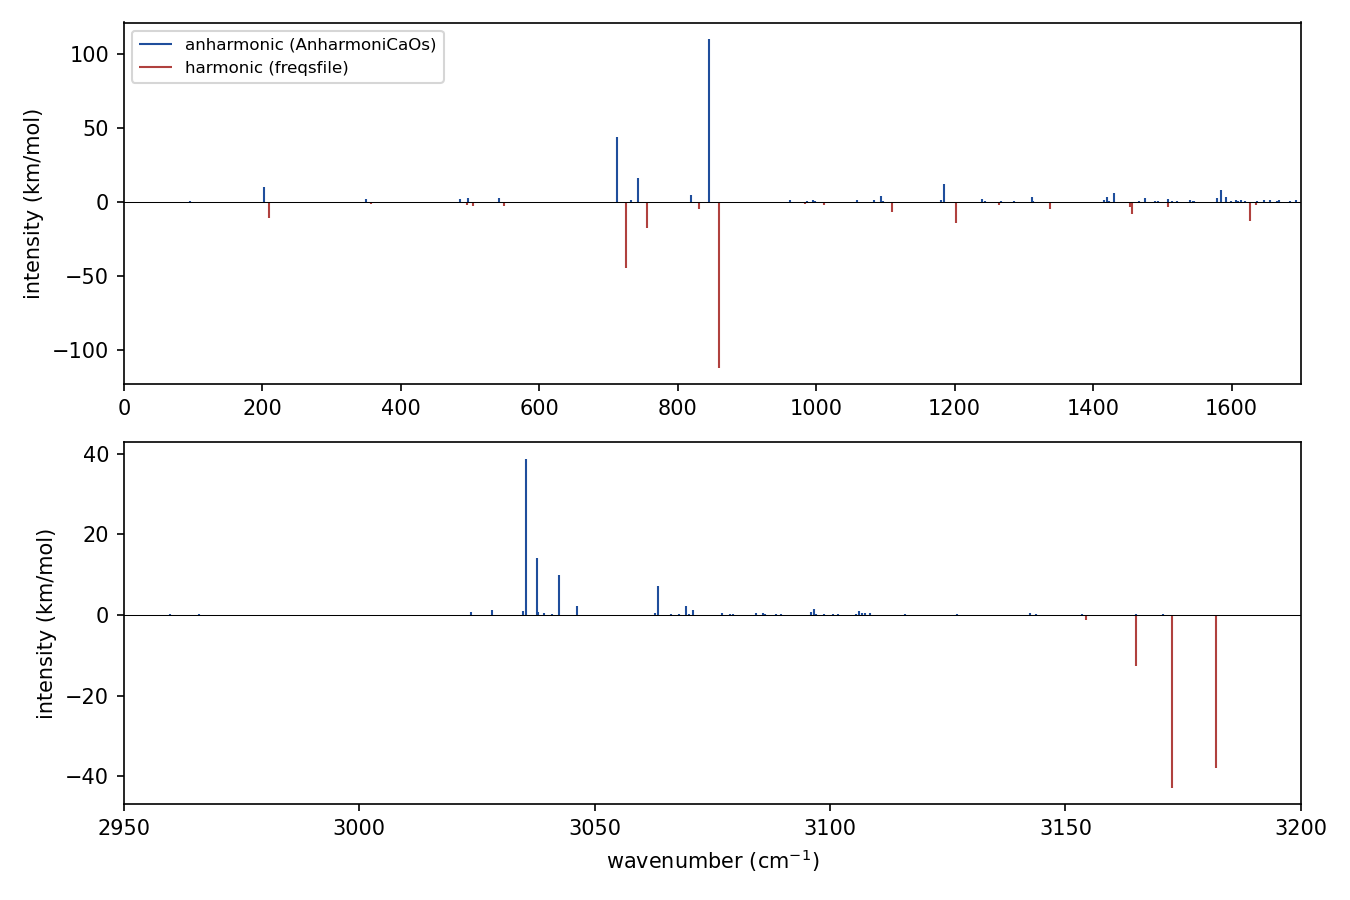
\includegraphics[width=\textwidth]{figures/pyrene-spectrum.png}
\caption{Pyrene, absorption from the ground state: the lines computed in
this tutorial (up) against the harmonic fundamentals of \file{freqsfile}
(down). The CH stretches (lower panel) move down by about 140~cm$^{-1}$ and
split among the states they are in resonance with.}
\label{fig:pyrene}
\end{figure}

These numbers and the figure come from a run of \file{run.sh} with
AnharmoniCaOs 2026.11.1 (\texttt{git 88b3b13}, the release candidate; the
programs of the release are the same) on a 4-core laptop.

\subsection*{Choice of the eigensolver}

\opt{eigensolver} selects the library that diagonalises the polyads in
phase 2b:
\begin{itemize}
\item \texttt{2}, ScaLAPACK \texttt{pdsyevx}: used in all the tutorials;
\item \texttt{1}, ScaLAPACK \texttt{pdsyevr}: same spectra;
\item \texttt{0}, SLEPc: the lines it finds agree with ScaLAPACK, but
  some weak lines are missing (on the same input with \opt{hsizescalepar}~=~4,
  1439 lines and 2\% of the total intensity); the reason is being
  investigated;
\item \texttt{3}, ELPA: same spectra (relative L1 distance below
  $10^{-7}$, the same transition energies), and the fastest. Its two-stage
  solver (\opt{elpasolver}~=~2) needs blocks of at most 64
  (\opt{elpablock}); with blocks of 300 it gave wrong eigenvalues on the
  polyads of 3400 states and more, without any error.
\end{itemize}

Wall time of phase 2b of this tutorial on a 4-core laptop, with
AnharmoniCaOs 2026.11.1 (\texttt{git 88b3b13}); the three runs give the
same total, 446.08~km/mol:
\begin{center}
\begin{tabular}{lrr}
\hline
eigensolver & processes $\times$ threads & wall time \\
\hline
\texttt{pdsyevx} (2) & $4\times1$ & 1:05 \\
ELPA one-stage (3) & $1\times1$ & 0:27 \\
\opt{spectral}~$=1$, \opt{spectralexactmax}~$=3000$ & $1\times4$ & 0:06 \\
\hline
\end{tabular}
\end{center}
On polyads of this size more processes do not help: the cost of
distributing the matrices exceeds the gain, and one process with ELPA, or
several independent runs, is the efficient choice. The spectral method
(option \opt{spectral}) is fastest; with \opt{spectralexactmax} as
large as the largest polyad all the polyads are diagonalised exactly and
the spectrum agrees with the other solvers within its resolution
(relative L1 distance 0.5\%).

\section{Variations}

The same run with the options of Chapter~\ref{ch:inputs}:
\begin{itemize}
\item \opt{shiftgeometry}: lines shift by up to about 3~cm$^{-1}$, and some
  intensities change by 10--30\%;
\item \opt{closureterms}: only weak lines change;
\item \opt{dipole3}: the CH stretches go from 7.5\% to 10.3\% of the total
  intensity.
\end{itemize}

\chapter{Tutorial 2: from a Gaussian anharmonic calculation}\label{ch:tut-gaussian}

This tutorial starts from the output of a Gaussian
\texttt{freq=(anharmonic,...)} calculation, here for
1,2,3,6,7,8-hexahydropyrene (90 modes, B3LYP-D3/6-31G). The Gaussian input
and the compressed output are in \file{examples/hexahydropyrene}; the
same calculation is published in the PAH database of INAF--OACa,
\url{https://cosmicpah-qcals.oa-cagliari.inaf.it}. The route section is
\begin{lstlisting}
#p geom=check freq=(ReadFC,anharm,PrintDerivatives) b3lyp/gen/auto
   int=(grid=superfine) cphf=(grid=superfine) densityfit
   empiricaldispersion=gd3 iop(7/33=1,99/5=0) scf=xqc
\end{lstlisting}
The essential keywords are \texttt{freq=(anharm,PrintDerivatives)}, which
prints the cubic and quartic force constants and the dipole derivatives
in normal coordinates. \texttt{ReadFC} and \texttt{geom=check} reuse a
previous optimisation and frequency calculation.

\section{Converting the Gaussian output}

\begin{lstlisting}
xz -dk 1_2_3_6_7_8-hexahydropyrene_distort1b.log.xz
python3 tools/gaussian2ac.py 1_2_3_6_7_8-hexahydropyrene_distort1b.log
\end{lstlisting}
The script writes \file{freqsfile}, \file{phi3file}, \file{phi4file},
\file{dmu2file} and, when the log contains them, the semidiagonal third
derivatives of the dipole (\file{dmu3file}, used with \opt{dipole3}). The
modes are renumbered by increasing wavenumber.

\section{Comparing with Gaussian}

\file{dunhamparams} uses the same convention as Gaussian's
``Total Anharmonic X Matrix'': each pair $i\le j$ is counted once.
Gaussian's matrix includes the Coriolis contributions, which \ac{}
neglects. Once these are subtracted, the two agree to the printed
precision, except for the entries that Gaussian deperturbs for its Fermi
resonances (129 of 4095 for this molecule). The zero-point energy agrees
to 0.03~cm$^{-1}$.
% TODO: script for this comparison; tables of fundamentals vs GVPT2.

\chapter{Tutorial 3: hot bands and emission at a given temperature}\label{ch:tut-thermal}

% TODO: sampling of the starting states (Monte Carlo / thermal), weights
% and nrepeats, energy bins (Ehist*), anharmonic energy histograms;
% splitting the work into parts and jobs (doc/polyad-jobs.md, T1/T2);
% example on pyrene at a moderate temperature with a small sample.
This chapter will show how to compute the spectrum of molecules with a
given internal energy or temperature, by averaging over a sample of
starting states, and how to split the work into cluster jobs.

The temperature enters through \opt{kT}, in cm$^{-1}$. It is convenient to
give the temperature in kelvin as a variable (Section~\ref{sec:inp}):
\begin{lstlisting}
temperature = 500        # K
kT = 0.6950348*temperature
\end{lstlisting}

\chapter{Tutorial 4: aiming at one band}\label{ch:tut-review}

Suppose that a weak observed band could be a dark band of the calculation,
but the computed intensity does not match. This tutorial shows how to
recompute only what concerns that band, more accurately, without
repeating the whole calculation.
\begin{enumerate}
\item In \file{resonancecandidates}, find the quantum-number changes that
  involve the dark state. Lines marked \texttt{near} are close to a
  threshold. Set their last column to \texttt{on}.
\item In \file{bandlist}, leave active only the band of interest (and the
  bright band it borrows from), setting the others to \texttt{off}.
\item Rerun phase 1 with
\begin{lstlisting}
resonanceoverrides = "resonancecandidates"
bandlistfile = "bandlist"
\end{lstlisting}
  then phases 2a and 2b, only for the starting states that matter.
\end{enumerate}
% TODO: worked example on pyrene with numbers.

\chapter{Input reference}\label{ch:inputs}

\section{Conventions}

The code uses the following conventions \notes{§2}:
\begin{itemize}
\item dimensionless normal coordinates, $q=(a+a^\dagger)/\sqrt2$;
\item energies in cm$^{-1}$;
\item $H=\sum\omega(p^2+q^2)/2+\frac{1}{3!}\sum\Phi_{ijk}q_iq_jq_k
  +\frac{1}{4!}\sum\Phi_{ijkl}q_iq_jq_kq_l$;
\item dipole derivatives in atomic units.
\end{itemize}
Indices in the files are 1-based. Force constants can be given for any
order of the indices; each distinct set of indices must appear once.

\section{The options file \file{inp}}\label{sec:inp}

All three programs read their options from \file{inp} with the
\texttt{oct\_parser} library, the input parser of the Octopus code
(included as the submodule \file{external/oct-parser}). This has some
practical consequences.

\begin{itemize}
\item \emph{Syntax.} One option per line, \texttt{name = value}; strings in
  double quotes; \texttt{\#} starts a comment; a line ending with
  \texttt{\textbackslash} continues on the next one. Names are not case
  sensitive.
\item \emph{Defaults.} Every option has a default, and only the options
  that differ from it need to be given. The defaults are listed in
  \file{README.md} of the code.
\item \emph{\file{out.oct}.} Each program writes to \file{out.oct} every
  option it has read, with the value it used. Values not given in
  \file{inp} are marked \texttt{\# default}. This is the place to check
  what a run actually used. Each program overwrites the file, so copy it
  after each phase if you want to keep all three (as \file{run.sh} of the
  tutorials does).
\item \emph{Misspelled options.} A misspelled option name is not an error:
  the parser takes it as a variable of its own, and the program uses the
  default. Check \file{out.oct} when an option seems to have no effect.
\item \emph{Variables and arithmetic.} Any name that is not an option can
  be used as a variable, and values can be expressions with the usual
  operators and functions (\texttt{sqrt}, \texttt{exp}, \texttt{log},
  \ldots) and the constants \texttt{pi} and \texttt{e}. A variable must be
  defined before it is used. The names \texttt{x}, \texttt{y}, \texttt{z},
  \texttt{r}, \texttt{w}, \texttt{t} and \texttt{i} are reserved (case
  insensitive) and cannot be used as variables. For example:
\begin{lstlisting}
thres = 0.20             # a variable, not an option
fermithres = thres
ddthres = thres
temperature = 500        # K
kT = 0.6950348*temperature   # kT is in cm-1
\end{lstlisting}
\end{itemize}

\section{Files}

\begin{description}
\item[\file{freqsfile}] One line per mode: $\omega$, then
  $\partial\mu/\partial q$ ($x$, $y$, $z$), then two optional columns: a
  legacy scale factor (unused) and a flag. In the release, a flag of 1
  computes the fundamental of that mode and 0 disables it; a disabled mode
  also has its dipole derivative set to zero. \devonly{} The flag is
  ignored, with a warning, and the bands are chosen in \file{bandlist}.
\item[\file{phi3file}, \file{phi4file}] Lines \texttt{i j k value} and
  \texttt{i j k l value}. Entries below \opt{phi3threshold} and
  \opt{phi4threshold} (cm$^{-1}$) are dropped.
\item[\file{dmu2file}] Lines \texttt{i j dx dy dz}: second derivatives of
  the dipole.
\item[\file{dmu3file}] Optional, with \opt{dipole3}: lines
  \texttt{i j k dx dy dz}. Missing entries are taken as zero.
\item[\opt{modepopfile}] Starting states: the quantum numbers of all modes,
  then the repetition count.
\item[\opt{gradientfile}] Optional: the classical gradient at the reference
  geometry, lines \texttt{i g\_i} (written by \opt{shiftgeometry}).
\item[\opt{bandlistfile}, \opt{resonanceoverrides}] \devonly{} Edited copies of
  \file{bandlist} and \file{resonancecandidates}
  (Chapter~\ref{ch:tut-review}).
\end{description}

\section{Options}

% TODO: generate this section from a single machine-readable table, shared
% with README.md, so that the two cannot diverge.
\subsection*{Resonances}
\begin{description}
\optentry{fermithres}{0.2}{1}{Threshold on $|W/\Delta|$ for cubic (Fermi) resonances.}
\optentry{ddthres}{0.2}{1}{The same for quartic (Darling--Dennison) resonances.}
\optentry{samesignresonances}{0}{1}{Also accept terms whose detuning is a single frequency.}
\optentry{closureterms}{0}{1}{Add the closure terms $-P[S_1,PH_1]$ to the resonant couplings \notes{Eq.~163}.}
\optentry{rescriterion}{0}{1}{\devonly{} 1: decide resonances from the error of perturbation theory on energies (\opt{resenergythres}, cm$^{-1}$, following~\cite{martin1995}) and relative intensities (\opt{resintensityrel}, \opt{resdarkrel}, \opt{resdarkmin}), up to \opt{rescheckquanta} quanta.}
\optentry{resonanceoverrides}{""}{1}{\devonly{} Force resonances on or off (Chapter~\ref{ch:tut-review}).}
\end{description}
\subsection*{Geometry and dipole}
\begin{description}
\optentry{shiftgeometry}{0}{1}{Move the reference geometry to remove the linear terms; writes the shifted force field (\file{*.shifted}).}
\optentry{dipole3}{0}{1}{Third-order transformed dipole for fundamentals and hot bands.}
\end{description}
\subsection*{Bands}
\begin{description}
\optentry{bandthres}{see README}{1}{Default activation of overtone, combination and difference bands, by $|\partial^2\tilde\mu|$.}
\optentry{fundthres}{1e-6}{1}{\devonly{} Default activation of fundamentals, by $|\partial\mu|$. A dipole derivative below it is numerical noise of a symmetry-forbidden mode and is set to zero when \file{freqsfile} is read.}
\optentry{bandlistfile}{""}{1}{\devonly{} Edited band list. It is read at the start of phase 1: an unknown choice stops the run at once, and lines that match no listed band give a warning.}
\end{description}
\subsection*{Checks}
\begin{description}
\optentry{dunhamcheck}{1}{1}{Stop if a deperturbed level falls at or below a lower one (Chapter~\ref{ch:trouble}).}
\optentry{dunhamfix}{0}{1}{Make the near Fermi resonances responsible explicit.}
\optentry{residualcheck}{0}{2b}{Estimate the truncation error of the polyads.}
\end{description}
\subsection*{Polyads and diagonalisation}
\begin{description}
\optentry{hsizescalepar}{see README}{2a}{Scale of the polyad growth.}
\optentry{maxtothops}{see README}{2a}{Maximum number of resonant steps.}
\optentry{costmodel}{0}{2a}{\devonly{} Cost of one resonant step when a polyad grows: 0, $1/\max(1.5,\ \opt{hsizescalepar}\,|W/\Delta E|)$; 1, $1/(\opt{costscale}\,|W/\Delta E|+1)$. Both at least $1/\opt{maxtothops}$.}
\optentry{costscale}{6}{2a}{\devonly{} Scale for \opt{costmodel}~$=1$, calibrated on toy Fermi and Wannier--Stark ladders (\file{tools/costmodel\_toy.py}).}
\optentry{minhopcoupling}{0.5}{2a}{\devonly{} A polyad does not grow through a coupling $|W|$ below this value (cm$^{-1}$); the coupling stays in the matrix when both states are in the polyad. Set it to 0 to switch it off and get the polyads of earlier versions.}
\optentry{eigensolver}{1}{2b}{Diagonalisation library: 1 ScaLAPACK \texttt{pdsyevr}, 2 ScaLAPACK \texttt{pdsyevx}, 0 SLEPc, 3 ELPA (the fastest in the tests of Chapter~\ref{ch:tut-pyrene}). With 1 and 3, the small polyads (at most 300 states per row or column of the process grid beyond the first) go to \texttt{pdsyevx}.}
\optentry{elpasolver}{1}{2b}{With \opt{eigensolver}~=~3: ELPA's one-stage (1) or two-stage (2) solver.}
\optentry{elpablock}{64}{2b}{With \opt{eigensolver}~=~3: block size of the distributed matrices. ELPA's two-stage solver gives wrong eigenvalues, without any error, with large blocks (it did with 300); keep it at 64 or below. Its GPU kernel needs a power of 2. See Section~\ref{sec:elpa}.}
\optentry{spectral}{0}{2b}{Kernel polynomial (spectral) method for large polyads; resolution \opt{spectraldelta}.}
\optentry{groundtransitions}{0}{2b}{\devonly{} With \opt{computeground}~$=1$: in the ground-state step, which adds nothing to the spectra, diagonalise all its polyads and compute the lines of the ground state, which \texttt{groundlines} (\opt{verbosity} bit 4) writes. With 0 only the polyad of the ground state is diagonalised, for the reference energy, and \texttt{groundlines} gives a warning instead of the lines. It applies to every \opt{eigensolver} and to \opt{spectral}. It does not change the spectra. Its older name, \opt{spectraleigenground}, is still read.}
\optentry{spectralexactmax}{0}{2b}{\devonly{} With \opt{spectral}~$=1$: a starting polyad of at most this many states is diagonalised, and its eigenstates replace the energy windows of the starting state (much faster for starting states in small polyads, such as the ground state). The destination polyads are still treated spectrally. Changes the spectra within the resolution; 0 switches it off.}
\end{description}
\subsection*{Histograms}
\begin{description}
\optentry{wnumhistmin, wnumhistmax, wnumhiststep}{}{2b}{Wavenumber grid (cm$^{-1}$).}
\optentry{Ehistmin, Ehistmax, Ehiststep}{}{2b}{Bins of the energy of the starting state.}
\end{description}
\subsection*{Log output}
\begin{description}
\optentry{verbosity}{0}{all}{What the logs (\file{proclog\_n*}) contain. It is a sum of the bits of Table~\ref{tab:verbosity}, which can be given by name: for example \texttt{verbosity = timings + components} instead of \texttt{verbosity = 10}. Write each name once: a name written twice adds its bit twice, which gives another bit. \opt{verbosity} does not change the spectra. In the released version bit 4 also changes what phase~2a builds: without it, phase~2a builds no polyads of the band destinations, and the spectra are empty, so keep bit 4 set there. \devonly{} In the development version \opt{verbosity} never changes what is computed; the lines of the ground state need \opt{groundtransitions}~$=1$.}
\end{description}
\begin{table}[ht]
\centering
\caption{Bits of \opt{verbosity}.}\label{tab:verbosity}
\begin{tabular}{rlp{0.62\textwidth}}
\hline
bit & name & what is written \\
\hline
1 & \texttt{polyadlevels} & For each starting state, the basis states of its polyads, with the target states marked by \texttt{*}, and their levels. With \opt{spectral}~$=1$, a polyad that is not diagonalised says so and lists only its basis states; a starting polyad diagonalised with \opt{spectralexactmax} lists its eigenstates and their weight on the starting state. \\
2 & \texttt{timings} & Timings and polyad sizes. With \opt{spectral}~$=1$, the summary lines \texttt{spectral:}, \texttt{spectral border:} and \texttt{spectral timing:} for each starting state. \\
4 & \texttt{groundlines} & The lines of the ground state, with their assignment. In the released version this bit also makes phase~2a build the polyads of the band destinations. \devonly{} The lines need \opt{groundtransitions}~$=1$. \\
8 & \texttt{components} & The main components of the eigenstates. \\
16 & \texttt{transitions} & Every transition. \\
32 & \texttt{spectraldiag} & \devonly{} Internals of the spectral method: one line per energy window of the starting state, and one per destination polyad, with its size, Chebyshev parameters and wall time. \\
\hline
\end{tabular}
\end{table}

\chapter{Output reference}\label{ch:outputs}

\section{Phase 1}
\begin{description}
\item[\file{resonanceslist}] One line per resonant term: type (B3, D4, E4,
  G2, \ldots), modes, coupling, detuning and their ratio.
\item[\file{dunhamparams}]\label{sec:dunham} The deperturbed expansion
  $E(n)=E_0+\sum_i w_i(n_i+\frac12)+\sum_{i\le j}x_{ij}(n_i+\frac12)(n_j+\frac12)$,
  with each pair counted once, as in Gaussian's X matrix. It gives $E_0$,
  the zero-point energy, $\omega_i$, $w_i$, the deperturbed fundamentals
  $\nu_i$, and all the $x_{ij}$. In the theory notes the sum runs over
  ordered pairs, so $x_{ij}=2\chi_{ij}$ for $i\ne j$ \notes{§6.6}.
\item[\file{bandlist}] \devonly{} All bands with their dipole derivative, harmonic
  wavenumber, intensity estimate and direction (\texttt{both}, \texttt{up},
  \texttt{down}, \texttt{off}).
\item[\file{resonancecandidates}] \devonly{} All candidate resonances with their
  metrics, decision and reason, grouped by change of quantum numbers. Terms
  that are resonant only because another term with the same change is
  (they are ``carried along'') are marked \texttt{carried}, so that the
  terms with decision~1 are exactly those of \file{resonanceslist}. The
  last column is the override in force (\texttt{on}, \texttt{off}) or
  \texttt{auto}.
\item[\file{*.shifted}, \file{gradient.shifted}, \file{shiftgeometry.out}]
  With \opt{shiftgeometry}.
\item[\file{dumpedparams}] Binary, read by phases 2a and 2b. It must come
  from the same version of phase 1.
\end{description}
\section{Phase 2a}
\begin{description}
\item[\file{dir\_nNNNNN}] One directory per starting state, with the
  polyad structures and Hamiltonians.
\item[\file{processedquantas}, \file{processeddirs}] The starting states
  and their directories.
\item[\file{polyadsizes}] The polyad sizes.
\end{description}
\section{Phase 2b}
\begin{description}
\item[\file{hist\_abs\_0}, \file{\_1}, \file{\_2}, \file{hist\_ems\_*}]
  Absorption and emission histograms, one file per Cartesian component of
  the dipole, binned in wavenumber and in the harmonic energy of the
  starting state. The total spectrum is the sum of the three files.
\item[\file{hist\_anh\_*}] The same, binned in the anharmonic energy of the
  starting state.
\item[\file{hist\_energy}, \file{hist\_anhenergy}] Number of starting
  states per energy bin.
\item[\file{proclog\_n*}] Logs of each process, with the truncation
  estimates when \opt{residualcheck} is on.
\end{description}
% TODO: units and normalisation of the histograms; script to convert them
% into a spectrum in km/mol.

\chapter{Warnings and errors}\label{ch:trouble}

\begin{description}
\item[\texttt{steps of the deperturbed Dunham ladders are <= 0}] An
  excited level lies at or below a lower one. The log (\texttt{\#
  dunhamcheck:}) names the responsible constant and the cubic terms behind
  it.
  \begin{itemize}
  \item Type a (near Fermi resonance): use \opt{dunhamfix}~$=1$.
  \item Type b (a low-frequency, large-amplitude mode): use
    \opt{shiftgeometry}~$=1$ or \opt{samesignresonances}~$=1$.
  \end{itemize}
  See \notes{§11.8}.
\item[\texttt{rotatedcomp is ... > .5}] Some band mixes strongly with
  other states through terms treated as nonresonant, so its intensity is
  less accurate. The next line names the largest such term,
  with its harmonic detuning. If that detuning is small, make the term
  resonant: lower \opt{fermithres} (with \opt{rescriterion}~$=0$), or set its change to \texttt{on} in
  \file{resonancecandidates} and give the file back with
  \opt{resonanceoverrides}. With \opt{shiftgeometry} the rotation of the
  normal modes can also cause it.
\item[\texttt{freqsfile disables N modes in its 6th column}] That column
  was the choice of the fundamentals before 2026.11.1; it is now ignored.
  Choose the bands in \file{bandlist}.
\item[\texttt{error reading updown for band}] \file{dumpedparams} was
  written by the phase 1 of an older version. Rerun phase 1.
\item[\texttt{resintensitythres is no longer used}] Replace it by
  \opt{resintensityrel}.
\end{description}

\bibliographystyle{unsrt}
\bibliography{manual}
\end{document}
